\section{Introduction}
\label{intro}
The field of Reinforcement Learning is progressing further and further. A lot of algorithms have been published over the past years using various approaches to solve blackbox problems \cite{Wierstra14}. For this project we have been assigned the task to implement the Natural Policy Gradient (NPG) \cite{Rajeswaran2017,Kakade2001} and the Natural Evolution Strategies (NES) \cite{Wierstra14}. To evaluate their performance we also have been assigned two platforms, the Cartpole and the Furuta Pendulum. Three tasks have to be solved on these platforms including the Cartpole swing up, the Cartpole double pendulum stabilization and the Furuta pendulum swing up \cite{Furuta1991}. We will discuss these platforms and tasks further in \ref{plats} to show how they work. In this report we will shortly introduce the algorithms and platforms and present our results and findings.

\subsection{Algorithms}
\label{algos}
Reinforcement Learning can be defined by various different optimization problems. One of them is to use a trajectory based approach.
\begin{align}
  J(\pi) = \int_{\mathbb{T}} p^{\pi}(\tau) r(\tau) d\tau
\end{align}
By formulating the derivatives and applying the logarithm likelihood trick we can derive the "vanilla gradient" or REINFORCE algorithm \cite{Williams1992}
\begin{align}
  \nabla_{\theta} J(\pi) = \int_{\mathbb{T}} p^{\pi}(\tau) \nabla_{\theta} \log p^{\pi}(\tau) r(\tau) d\tau \approx \frac{1}{N} \sum_{i=1}^{N} \nabla_{\theta} \log p^{\pi}(\tau_i) r(\tau_i)
\end{align}
If we now add a constraint to regularize the gradients we can rewrite the optimization problem as
\begin{align}
  \max_{\delta\theta} \hat J(\theta + \Delta\theta) &= J(\theta) + \nabla_{\theta} J^T \Delta\theta \nonumber \\
  s.t. \ D(p_{\theta + \Delta\theta} || p_{\theta}) &= \Delta\theta^T F(\theta) \Delta\theta \leq \epsilon \label{NpgOpti}
\end{align}
with $F$ being defined to be
\begin{align}
  F = \frac{1}{T} \sum_{t=0}^{T} \nabla_{\theta} \log \pi_{\theta}(a_t | s_t)
  \nabla_{\theta} \log \pi_{\theta}(a_t | s_t)^T
\end{align}
This leads to the natural gradient in \cite{Rajeswaran2017}
\begin{align}
  \Delta \theta = \alpha F^{-1} \nabla_{\theta} J = \sqrt{\frac{\delta}{\nabla_{\theta} J^T F^{-1} \nabla_{\theta} J}} F^{-1} \nabla_{\theta} J
\end{align}
As a first setup we implemented the NPG as described in \cite{Rajeswaran2017} which however lead to a lot of problems while calculating the fisher information matrix (FIM). Not only is calculating the fisher matrix very computationally expensive, it can also result in uninvertable matrices \cite{DuanCHSA16}. To get around calculating the FIM directly we decided to use conjugate gradients to compute the natural gradient \cite{DuanCHSA16}. To further increase the efficiency we also added importance sampling through which we basically ended up implementing the Trust Region Policy Optimization \cite{SchulmanLMJA15,Telesens}. In this context we switched to neural network based policy representing a gaussian distribution. To prevent confusion we will still denote to this as NPG in this report.\\

In contrast the NES algorithms utilize a search distribution over the parameters. Each episode a batch of sample policies $z$ is drawn from this distribution. These samples are used to run a trajectory which is evaluated with a fitness function $f$. We can formalize this as an optimization function
\begin{align}
  J(\theta) = \int f(z) \pi(z|\theta) dz
\end{align}
which leads to an estimate of the search gradients from samples $z_1 ... z_{\lambda}$
\begin{align}
  \nabla_{\theta} J \approx \frac{1}{\lambda} \sum_{k=1}^{\lambda} f(z_k) \nabla_{\theta} \log \pi(z_k|\theta)
\end{align}
with population size $\lambda$ \cite{Wierstra14}. \\
The first version we implemented was the Canonical NES \cite{Wierstra14}. Similar to the NPG it adds a constraint to the optimization to regularize the gradients as in  \autoref{NpgOpti}. However as already described above we ran into problems while calculating the FIM. To avoid the same struggles as in the NPG we devided to switch to another version of the NES called Seperable NES (SNES) \cite{Wierstra14}.
\\ ADD EXPLANATION OF SNES

\subsection{Platforms}
\label{plats}
The algorithms have to be tested and evaluated on at least three different tasks. Two of these, the Cartpole swing up and the double pendulum stabilization, are executed on the Cartpole platform. The third task runs on the Furuta Pendulum \cite{Furuta1991}. \\

The Cartpole is a fairly simply mechanical system. It basically is a sledge sitting on a rail which can move left and right. Connected to the sledge is a stiff rod swinging freely whenever the sledge moves \cite{Barto1983}. There are several variations of tasks that can be done on the Cartpole platform ranging from simple stabilization of a single rod to more complex tasks like stabilizing two, three or even four rods stacked on top of each other connected by free links. Even more complex is the swing up. Starting in a hanging position the rod has to be swung up and stabilizing afterwards. The complexity can be increased further by stacking more rods similar as before. \\

The Furuta Pendulum is a rotary inverted pendulum invented by Katsuhisa Furuta and his colleagues in 1991 \cite{Furuta1991}. It is an underactuated, non-linear system with a stiff rod attached to a single motor by a rigid link. The motor rotates the rod in a horizontal plane. Attached to the other end of the rod is a free link with a second rod perpendicular to the first. When the motor moves the first rod, the second one rotates in a vertical plane always perpendicular to the first rod. Compared to the cartpole system it provides multiple advantage such as using less experimental space and having fewer uncertanties in the mechanical transmission system \cite{Furuta1991}. The task here is to use the rotation of the motor to swing up the second rod and stabalize it. Similar to the cartpole the complexity could be increased by stacking more rods with free links onto the second one in the same direction.
\begin{figure*}
  \begin{minipage}{.5\textwidth}
    \centering
    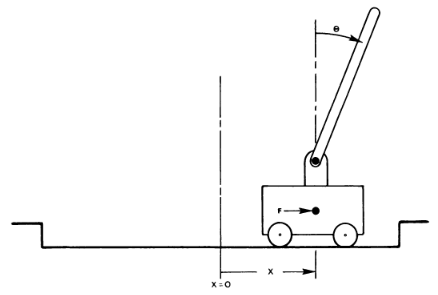
\includegraphics[scale=.3]{plots/Cartpole_model}
    \captionof{figure}{Cartpole Model \cite{Barto1983}}
    \label{fig:cartpole}
  \end{minipage}
  \begin{minipage}{.5\textwidth}
    \centering
    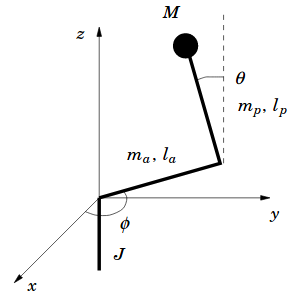
\includegraphics[scale=.3]{plots/Furuta_model}
    \captionof{figure}{Furuta Pendulum Model \cite{Lund}}
    \label{fig:furuta}
  \end{minipage}
\end{figure*}
